\begin{surferPage}[Octica Chmutov]{La Óctica de Chmutov}
    Una llamativa característica de la óctica de Chmutov ($\text{Chm}_{d}$ con $d=8$)
    es su simetría. Esto también puede ser visto observando su ecuación:
    \[\text{Chm}_{d}\colon T_d(x) + T_d(y) + T_d(z) + 1 = 0,\]
    donde $T_d$ es el polinomio de Tchebychev, cuyo gŕafico es el de la izquierda;
    y la curva $T_8(x)+T_8(y)=0$ está dibujada a la derecha:
    
     \begin{center}
      \begin{tabular}{c@{\quad}c}
        \begin{tabular}{c}
          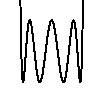
\includegraphics[height=1.75cm]{../../common/images/Tcheb_008.pdf}
        \end{tabular}    
        &
        \begin{tabular}{c}
          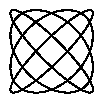
\includegraphics[height=1.75cm]{../../common/images/Tcheb_2d_008.pdf}
        \end{tabular}    
      \end{tabular}
    \end{center}
    \vspace{-0.3cm}
    Como puede verse, el paso desde estos gráficos a la forma de la superficie no es muy largo.
    
    Estas ecuaciones fueron dadas por Sergei Chmutov a principio de los 80's.
    En ese tiempo, tenían los récords mundiales de $\mu(d)$ para la mayoría
    de los valores de $d$. En los 90's, Chmutov mejoró su propio récord;
    y en 2005, Breske, Labs y van Straten adaptaron esta construcción para
    superficies reales con solamente singularidades reales.
\end{surferPage}
